\documentclass[tikz,border=3pt]{standalone}
\usepackage[T1]{fontenc}
\usepackage{newtxtext,newtxmath}
\usetikzlibrary{arrows.meta,calc}
\definecolor{ink}{HTML}{23343F}
\definecolor{teal}{HTML}{087F78}
\definecolor{orange}{HTML}{C46B2C}
\definecolor{blue}{HTML}{2276A0}
\definecolor{gray}{HTML}{4C5D67}
\definecolor{rule}{HTML}{D6DFE3}
\begin{document}
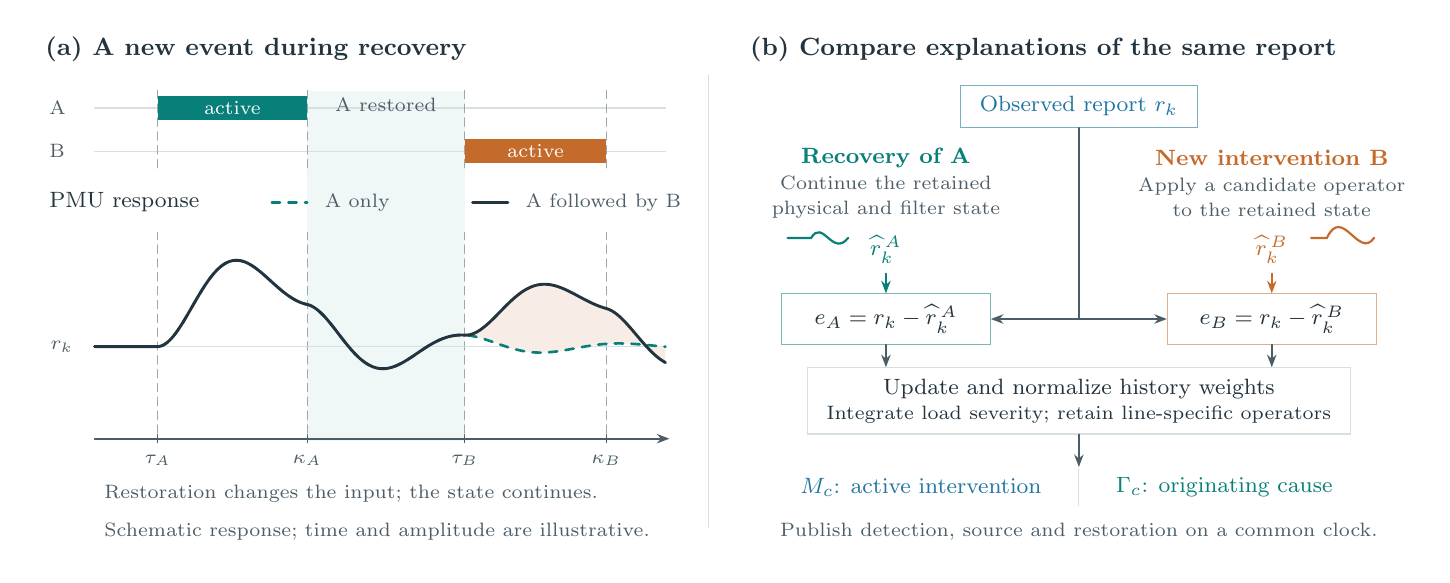
\begin{tikzpicture}[font=\fontsize{8.3}{10}\selectfont,text=ink,
 >={Stealth[length=1.6mm]},line cap=round,
 head/.style={anchor=west,font=\bfseries\fontsize{9.2}{11}\selectfont},
 small/.style={font=\fontsize{7.5}{9}\selectfont,text=gray},
 flow/.style={->,draw=gray,line width=.6pt},
 block/.style={draw=rule,fill=white,minimum height=.48cm,inner xsep=7pt,inner ysep=4pt}]
\path[use as bounding box] (0,0) rectangle (17.7,6.7);
\node[head] at (.1,6.42) {(a) A new event during recovery};
\node[head] at (9.05,6.42) {(b) Compare explanations of the same report};
\draw[rule] (8.65,.35)--(8.65,6.1);
% All pulse edges, trace onsets and clock labels share these coordinates.
\def\ta{1.65}\def\ka{3.55}\def\tb{5.55}\def\kb{7.35}
\fill[teal!6] (\ka,1.45) rectangle (\tb,5.9);
\node[small,anchor=west] at (.15,5.68) {A};
\node[small,anchor=west] at (.15,5.13) {B};
\draw[rule] (.85,5.68)--(8.1,5.68) (.85,5.13)--(8.1,5.13);
\fill[teal] (\ta,5.53) rectangle (\ka,5.83);
\fill[orange] (\tb,4.98) rectangle (\kb,5.28);
\node[text=white,font=\fontsize{7}{8}\selectfont] at (2.6,5.68) {active};
\node[text=white,font=\fontsize{7}{8}\selectfont] at (6.45,5.13) {active};
\foreach \xx in {\ta,\ka,\tb,\kb} {\draw[gray!55,densely dashed,line width=.4pt] (\xx,1.55)--(\xx,4.10) (\xx,4.92)--(\xx,5.94);}
\node[small] at (4.55,5.72) {A restored};
\node[anchor=west] at (.15,4.48) {PMU response};
\draw[teal,dashed,line width=.85pt] (3.1,4.48)--(3.55,4.48);
\node[small,anchor=west] at (3.65,4.48) {A only};
\draw[ink,line width=1pt] (5.65,4.48)--(6.1,4.48);
\node[small,anchor=west] at (6.2,4.48) {A followed by B};
\draw[rule,line width=.5pt] (.85,2.65)--(8.1,2.65);
\pgfmathdeclarefunction{step}{1}{\pgfmathparse{#1<0 ? 0 : 1-exp(-.65*#1)*(cos(180*#1)+.65/pi*sin(180*#1))}}
\pgfmathdeclarefunction{old}{1}{\pgfmathparse{.72*(step(#1-1.65)-step(#1-3.55))}}
\pgfmathdeclarefunction{new}{1}{\pgfmathparse{.57*(step(#1-5.55)-step(#1-7.35))}}
% Highlight the additional response, with both edges derived from the same clock.
\fill[orange!12] plot[domain=5.55:8.1,samples=100] (\x,{2.65+old(\x)+new(\x)})
 -- plot[domain=8.1:5.55,samples=100] (\x,{2.65+old(\x)}) --cycle;
\draw[teal,dashed,line width=.95pt] plot[domain=.85:8.1,samples=240] (\x,{2.65+old(\x)});
\draw[ink,line width=1.05pt] plot[domain=.85:8.1,samples=240] (\x,{2.65+old(\x)+new(\x)});
\node[small,anchor=east] at (.7,2.65) {$r_k$};
\draw[flow] (.85,1.48)--(8.15,1.48);
\foreach \xx/\lab in {\ta/{$\tau_A$},\ka/{$\kappa_A$},\tb/{$\tau_B$},\kb/{$\kappa_B$}} {
 \draw[gray] (\xx,1.43)--(\xx,1.53);
 \node[below,small] at (\xx,1.4) {\lab};
}
\node[small,anchor=west] at (.85,.78) {Restoration changes the input; the state continues.};
\node[small,anchor=west] at (.85,.3) {Schematic response; time and amplitude are illustrative.};
% Report travels down the central spine; predictor outputs enter separate scores.
\node[block,draw=blue!60,text=blue] (report) at (13.35,5.7) {Observed report $r_k$};
\node[text=teal,font=\bfseries\fontsize{8}{10}\selectfont] at (10.9,5.05) {Recovery of A};
\node[text=orange,font=\bfseries\fontsize{8}{10}\selectfont] at (15.8,5.05) {New intervention B};
\node[small,align=center] at (10.9,4.55) {Continue the retained\\physical and filter state};
\node[small,align=center] at (15.8,4.55) {Apply a candidate operator\\to the retained state};
\node[text=teal] (pa) at (10.9,3.88) {$\widehat r_k^{\,A}$};
\node[text=orange] (pb) at (15.8,3.88) {$\widehat r_k^{\,B}$};
\draw[teal,line width=.8pt] (9.65,4.03)--(9.95,4.03) .. controls (10.1,4.28) and (10.22,3.78) .. (10.42,4.03);
\draw[orange,line width=.8pt] (16.3,4.03)--(16.5,4.03) .. controls (16.7,4.45) and (16.9,3.75) .. (17.1,4.03);
\node[block,draw=teal!55,minimum width=2.65cm] (sa) at (10.9,3.0) {$e_A=r_k-\widehat r_k^{\,A}$};
\node[block,draw=orange!55,minimum width=2.65cm] (sb) at (15.8,3.0) {$e_B=r_k-\widehat r_k^{\,B}$};
\draw[flow,teal] (pa)--(sa);
\draw[flow,orange] (pb)--(sb);
\draw[gray,line width=.6pt] (report.south)--(13.35,3);
\draw[flow] (13.35,3)--(sa.east);
\draw[flow] (13.35,3)--(sb.west);
\node[block,minimum width=5.7cm,align=center] (norm) at (13.35,1.96)
 {Update and normalize history weights\\[-1pt]{\fontsize{7}{9}\selectfont Integrate load severity; retain line-specific operators}};
\draw[flow] (sa.south)--(sa.south |- norm.north);
\draw[flow] (sb.south)--(sb.south |- norm.north);
\draw[flow] (norm.south)--(13.35,1.12);
\node[anchor=east,text=blue] at (13.0,.86) {$M_c$: active intervention};
\node[anchor=west,text=teal] at (13.7,.86) {$\Gamma_c$: originating cause};
\draw[rule] (13.35,.63)--(13.35,1.1);
\node[small] at (13.35,.3) {Publish detection, source and restoration on a common clock.};
\end{tikzpicture}
\end{document}
